\section{Literature review}
\label{sec:literature-review}

The Wikipedia RfA process has been widely studied in various domains from many different perspectives such as those of the candidate, the voters and the community. In this section we discuss the existing work in this field.

Administrator is a highly coveted status on Wikipedia, and there are many features that can be used to determine the worthiness of a candidate. Wikipedia themselves provide tools and guides\footnote{http://en.wikipedia.org/wiki/Wikipedia:GRFA} to help potential candidate assess their own electability. For instance, Wikipedia's \textit{admin score tool} as seen in Figure~\ref{fig:admin-score} uses features such as edit counts, pages created, age of account etc. Similarly, Burke et al.\ \cite{BurkeMoppingUp} utilized data from past RfAs to find features that correlate highly with successful candidates such as presence of edit summaries, politeness in user interactions and varied experience. Such tools and models are useful for finding potential nominees and understanding what the community values and respects. This, however, does not offer any insights into the emergent dynamics in an election.
\begin{figure}[h!]
    \centering
    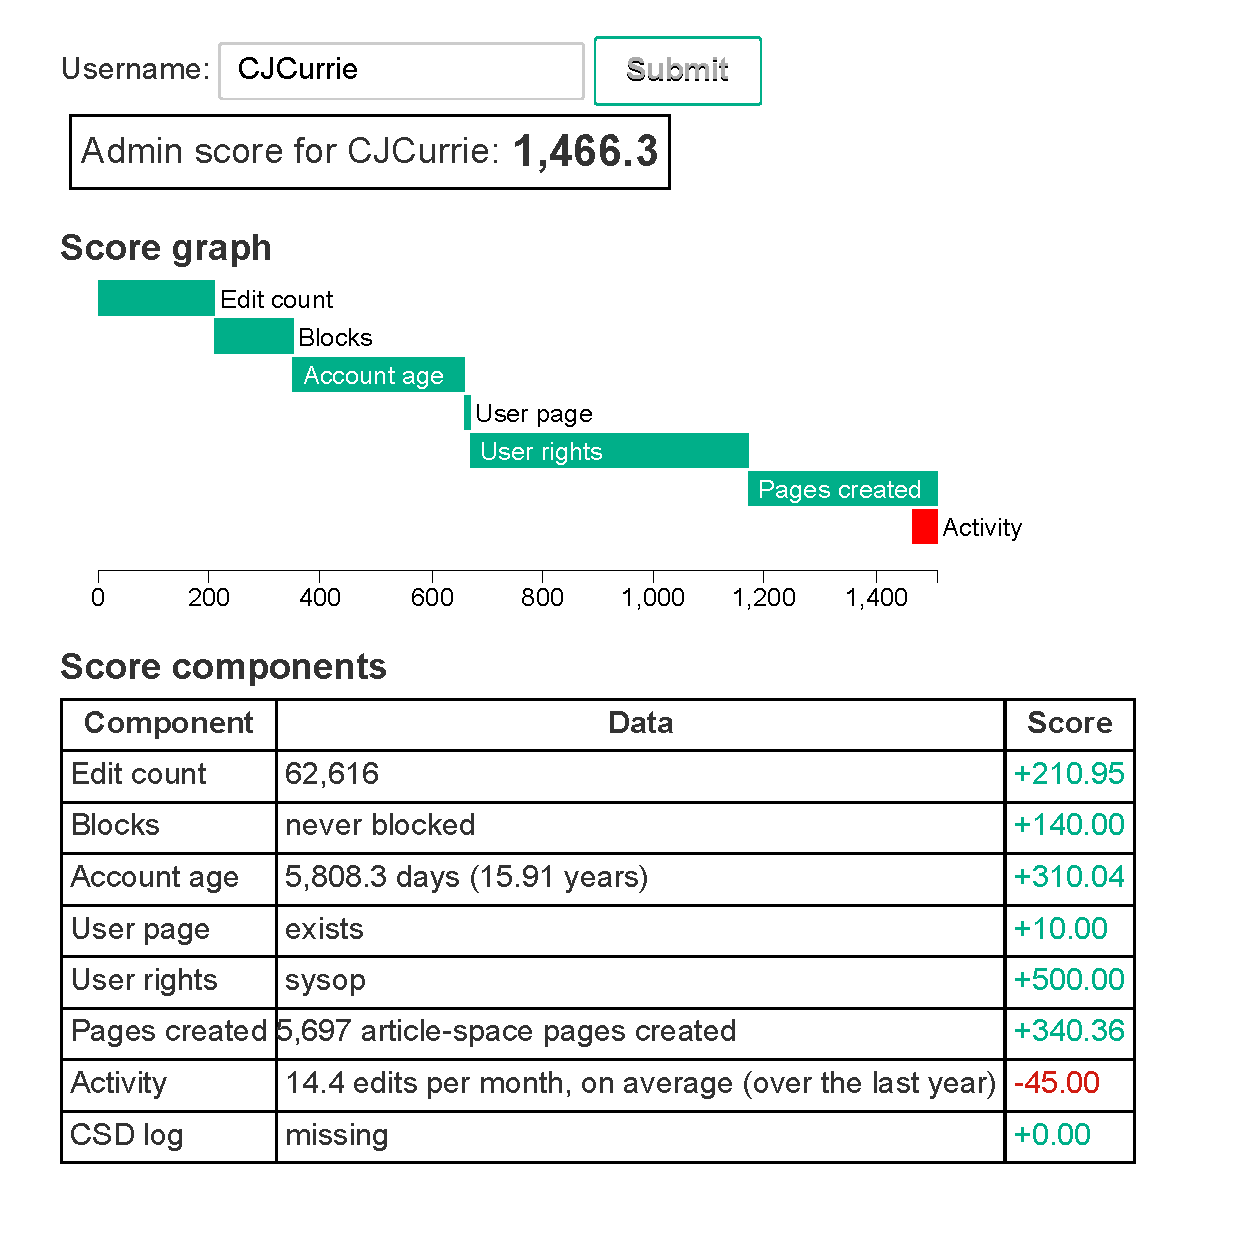
\includegraphics[width=\linewidth]{images/Asynchronous Admin Score.pdf}
    \caption{Admin score tool for user CJCurrie and its breakdown}
    \label{fig:admin-score}
\end{figure}

Leskovec et al.\ \cite{leskovec2010governance} provide a thorough analysis of the election from the perspective of the voter. They show that the voters make decisions based on \textit{relative assessment} of merit and degree of correspondence with the candidate. Moreover, voters do not follow a \textit{herd mentality} that is usually seen in other information cascade settings. We see an interesting result that voters have diverse personal response functions as well as admin and non-admin patterns of voting differ. Their work presents a detailed picture of the temporal dynamics in a RfA.

As the votes in an RfA election can be positive or negative, they can form a \textit{signed network}, which has been studied and analysed in great detail. For example, Leskovec et al.\ \cite{leskovecSigned} show that the Wikipedia RfA network is more compliant with status theory compared to balance theory. When they used structural properties of signed networks to predict edges, they observed that the predictive accuracy is poor for the Wikipedia RfA network compared to the other networks in their experiments. However, as signed edge prediction methods are designed to work with any generic signed network, they tend to discard information that RfAs are elections and occur chronologically. There are more works that propose different models and approaches to predicting singed links \cite{agrawal2013link,hsieh2012low,gu2019link,chiang2011exploiting,Jiliang2015Negative,chiang2014prediction}. Nevertheless, predicting a single edge or a vote in an election does not increase the accuracy when predicting the result of an election. In this paper, we aim to use the interactions within voters in the Wikipedia network to predict the eventual result of a RfA election.

The work of Desai et al.\ \cite{desai2014result} is related closely with the contributions presented in this paper. Their approach uses linear models for regression and classification to identify a core of \textit{influential voters} through feature selection. Therefore, using a set of 40 most influential voters, they are able to predict the result of an election with high accuracy. They also collect additional network features of the voters independent from the elections. The results do not improve significantly when using these additional features in predicting election results. These results show that there are a group of influential voters that determine election results. This will be more evident when we analyse the dataset in the coming sections.
